\subsection*{Objective}
In the previous experiments, the one-shot approach to food image
classification has been looked at. That is, the model will give a prediction of the most likely
food item in that image. This is a problem when there is a composite image i.e are multiple foods in an
image, see Figure \ref{fig:fruit}. There are a few options to combat this problem. Firstly, one could detect
objects in the image, segment the image according to these objects and then run
each segment through the model.
A simple approach to this would be to segment
the image into several sections and then run each section through the model.
To follow the latter approach, a sliding window approach was used. This
sliding window would move across the image and classify the segment of the image
in the window. There are three options for window sliding shape as defined by a
command line argument.

\begin{lstlisting}[style=Command]
python sliding_window.py --image=~/image_dir --window_shape grid
\end{lstlisting}

There are three options for window shape:
\begin{itemize}
	\item{Grid based window as per Figure \ref{fig:fruitGrid}}
	\item{Row based window as per Figure \ref{fig:fruitRow}}
	\item{Column based window as per Figure \ref{fig:fruitColumn}}
\end{itemize}

\begin{figure}
    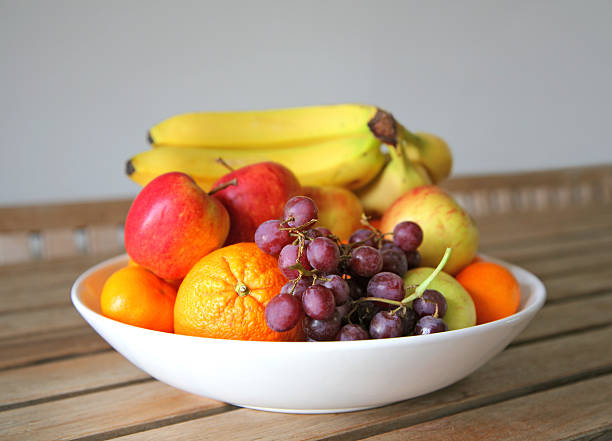
\includegraphics[scale=0.5]{fruit}
    \caption{Bowl of fruit - sourced from https://www.geo.de/natur/}
    \label{fig:fruit}
\end{figure}

\begin{figure}
    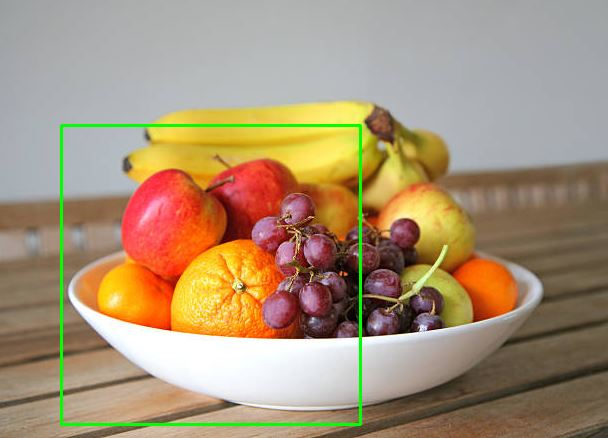
\includegraphics[scale=0.5]{fruitGrid}
	\caption{Grid based window}
    \label{fig:fruitGrid}
\end{figure}

\begin{figure}
    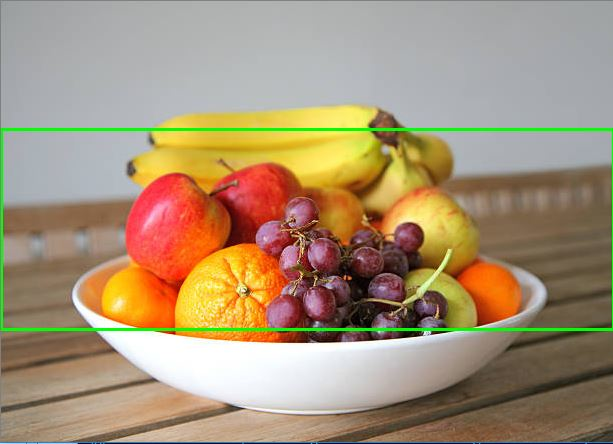
\includegraphics[scale=0.5]{fruitRow}
    \caption{Row based window}
    \label{fig:fruitRow}
\end{figure}

\begin{figure}
    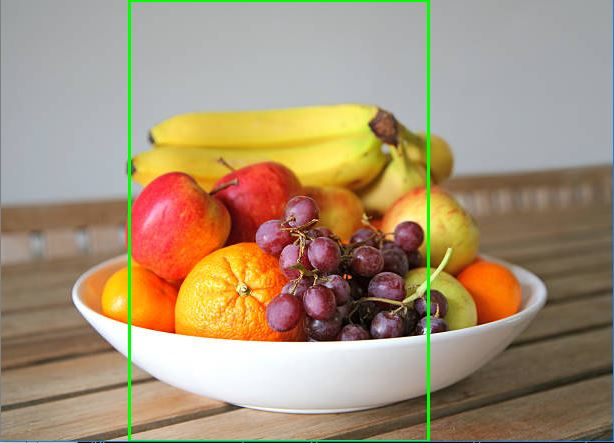
\includegraphics[scale=0.5]{fruitColumn}
    \caption{Column Based Window}
    \label{fig:fruitColumn}
\end{figure}

\begin{figure}
    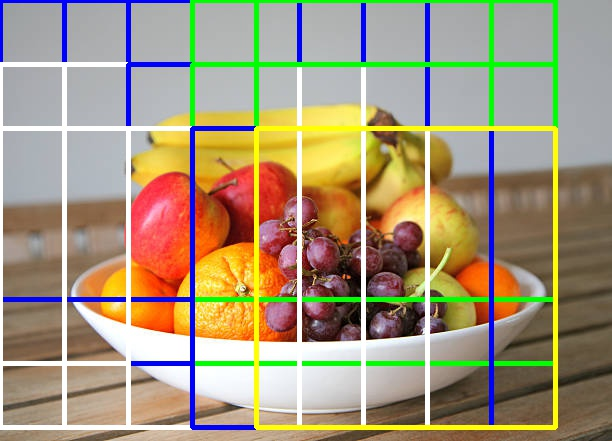
\includegraphics[scale=0.5]{fruitCO}
    \caption{Fruit with Color Overlay}
    \label{fig:fruitOverlay}
\end{figure}

\subsection*{Libraries}
For this experiment TensorFlow provided the classification of each segment while
also helping with resizing along with NumPy. OpenCV was used to implement the
sliding window as per \parencite{slidingWindowTut}.

\subsection*{Script}
There were four main elements to the script. Firstly, extracting a window to be
classified. Secondly, resizing the image to be compatible with the TensorFlow model. Thirdly, running the window through the TensorFlow model and finally
saving a new image with a coloured overlay of classifications.

\subsubsection*{Extracting the window from the image}
\begin{lstlisting}[style=Python]
for (x, y, window) in sliding_window(resized, stepSize=64, windowSize=(winW, winH)):
	# if the window does not meet our desired window size, ignore it
	if window.shape[0] != winH or window.shape[1] != winW:
		continue
\end{lstlisting}


\begin{lstlisting}[style=Python]
def sliding_window(image, stepSize, windowSize):
	# slide a window across the image
	for y in xrange(0, image.shape[0], stepSize):
		for x in xrange(0, image.shape[1], stepSize):
			# yield the current window
			yield (x, y, image[y:y + windowSize[1], x:x + windowSize[0]])
\end{lstlisting}

\subsubsection*{Resizing the window}
\begin{lstlisting}[style=Python]
window = cv2.resize(window, (299, 299))
\end{lstlisting}

\begin{lstlisting}[style=Python]
resized_image = tf.reshape(image, [1, input_height, input_width, 3])
resized = tf.image.resize_area(resized_image, [input_height, input_width])
normalized = tf.divide(tf.subtract(resized, [input_mean]), [input_std])
\end{lstlisting}

\subsubsection*{Running the Tensorflow model}
\begin{lstlisting}[style=Python]
with tf.Session() as sess:
	numpy_image = sess.run(normalized)

with tf.Session(graph=graph) as sess:
    results = sess.run(output_operation.outputs[0],
                      {input_operation.outputs[0]: numpy_image})
	probabilities = np.squeeze(results)
\end{lstlisting}

\subsubsection*{Saving the image with colour overlay}
As seen in Figure \ref{fig:fruitOverlay}, each square represents a window and
each colour is for a different classification. Blue is for an apple, yellow for
banana, green for grape, white for orange and black if an unexpected prediction
is made.

\begin{lstlisting}[style=Python]
cv2.rectangle(display_image, (x, y), (x + winW, y + winH), colour_dict.get(top1,
(0,0,0)), 4)
\end{lstlisting}

\subsection*{Results}
\subsubsection*{Grid based window}
The grid-based window resulted in fifteen separate classification. As seen in Figure
\ref{fig:fruit}, there are multiple fruits in the image. Of these fruits, our
model is trained on four, apple, banana, orange and grapes. This method
classified all four to Top-1 accuracy at least once each. This method took 42.8
seconds to run.

\begin{table}[]
	\centering
	\caption{Grid Based Sliding Window Results}
	\label{my-label}
	\begin{tabular}{|l|l|}
	\hline
		\textbf{Food type} & \textbf{No. of Top-1 Classifications} \\ \hline
		Apple     & 5                      \\ \hline
		Banana    & 1                      \\ \hline
		Grape     & 4                      \\ \hline
		Orange    & 5                     \\ \hline
	\end{tabular}
\end{table}

\begin{table}[]
	\centering
	\caption{Row Based Sliding Window Results}
	\label{rowWindowTable}
	\begin{tabular}{|l|l|}
	\hline
		\textbf{Food type} & \textbf{No. of Top-1 Classifications} \\ \hline
		Apple     & 1                      \\ \hline
		Banana    & 0                      \\ \hline
		Grape     & 0                      \\ \hline
		Orange    & 0                      \\ \hline
		Other     & 3                     \\ \hline
	\end{tabular}
\end{table}

\begin{table}[]
	\centering
	\caption{Column Based Sliding Window Results}
	\label{colWindowTable}
	\begin{tabular}{|l|l|}
	\hline
		\textbf{Food type} & \textbf{No. of Top-1 Classifications} \\ \hline
		Apple     & 3                      \\ \hline
		Banana    & 1                      \\ \hline
		Grape     & 0                      \\ \hline
		Orange    & 0                      \\ \hline
		Other     & 1                     \\ \hline
	\end{tabular}
\end{table}

\subsubsection*{Row based window}
The row-based method resulted in four predictions as follows in Figure
\ref{rowWindowTable}. Out of these four predictions, only one classified a known
fruit at Top-1 accuracy, an apple. An apple was also predicted to Top-5 accuracy
in another instance. The runtime of this method was 16.1 seconds.

\subsubsection*{Column based window}
The column-based window approach had five total predictions and ran for a total
of 13 seconds. As seen in \ref{colWindowTable}, two out of four known fruits
were classified to a Top-1 accuracy with all other fruits predicted to Top-5
accuracy. Only one Top-1 prediction did not contain a correct fruit.

\subsection*{Analysis}
These results are very interesting because while a banana was only predicted to
Top-1 accuracy once in grid based, once in column based and zero times in row
based, if the whole image is passed through the model, a banana is at the Top-1 accuracy.
























